\documentclass[a4paper,12pt]{article}
\usepackage[utf8]{inputenc}
\usepackage[frenchb]{babel}
\usepackage{graphicx}
\usepackage[T1]{fontenc}
\usepackage{fancyhdr}
\usepackage{graphics}
\usepackage{verbatim}
\usepackage{url}
\setcounter{page}{1}
\fancyhead[L]{\leftmark}
\fancyhead[R]{}

\fancyfoot[C]{}
\fancyfoot[R]{\thepage}



\begin{document}
\begin{titlepage}
		\newpage
		\thispagestyle{empty}
		\begin{center}
			
\includegraphics[scale=0.15]{images/logo_fac}	
		\end{center}
		\begin{center}
			\vspace{0.3cm}
			\large  
			\textbf{Mémoire de Master 2 MIAGE}\\
			\vspace{0.7cm} \large 
			\vskip 0.2in
		\end{center}
		\fbox{%
			\parbox{\textwidth}{%
				\begin{center}
					\begin{center}
						\large \textsc{\textbf{ Comment, à partir de la reconnaissance faciale et de la fouille de données, peut-on identifier l’ensemble des sosies potentiels d’une personne ?  }}
					\end{center}
					
				\end{center}
			}%
		}
		\begin{center}
		    Application à l’univers du cosplay
		\end{center}
		
		\begin{flushleft}
			\begin{center}
			
					\textbf{Réalisé par} \\
					\hspace{0.1cm} VILLER Nathanaëlle \\
					\textbf{Tuteur}\\
				 \hspace{0.1cm} GUEHIS Sonia \\
			
			\end{center}
		\end{flushleft}
	
		\begin{center}
			\vspace{0.1cm} \textbf{Année scolaire 2017-2018}
		\end{center}
		
%\newpage
%\thispagestyle{empty}
%\section*{Remerciements}
 
\newpage
\tableofcontents
\thispagestyle{empty}
\end{titlepage}

\newpage
	\pagenumbering{arabic}
%\addcontentsline{toc}{section}{Introduction}
%\section*{Introduction}

%\textit{}
%\\ \\

%\newpage

\addcontentsline{toc}{section}{Glossaire}
\newpage
\section*{Glossaire}
\begin{description}
\item [Sosie :] Personne qui a une parfaite ressemblance avec une autre au point qu'on peut les confondre.
\item [Cosplay :] Le phénomène du cosplay a commencé dans les années 40 aux États unis. Mais c'est lors des années 70 et 80 que le cosplay atteint son paroxysme grâce aux succès de Star Trek et Star Wars. Le Japon va ensuite adopter ce phénomène et lui donner le nom qu'il porte aujourd'hui : le cosplay (qui vient de la contraction de costume et playing). Le principe est simple : il faut se déguiser en un personnage de fiction et incarner ce personnage. Le mouvement va s'intensifier au Japon et Tokyo deviendra le centre névralgique de ce phénomène. Il faudra attendre les années 90 pour que le cosplay arrive en Europe. La scène européenne se démarquera par sa volonté de respect du craft (fabrication manuelle de son costume). Les conventions et concours vont se multiplier. Les cosplayers vont de plus en plus chercher de nouvelles techniques pour pouvoir ressembler le plus possible aux personnages qu'ils essaient d'incarner. Il y a 2 grandes catégories qui se démarquent. Ceux qui cosplay leurs personnages préférés sans se soucier de la morphologie et ceux qui essaie de trouver des personnages qui leur correspondent physiquement.
\item [Cosplayer :] n.m peut s'écrire aussi cosplayeur, ou cosplayeuse pour les femmes. Il s'agit d'une personne pratiquant l'art du cosplay. 
\item [Cosplayer :] Verbe d'action signifiant l'art de pratiquer le cosplay. 
\item [Crawler / Robot d'indexation :] Un robot d’indexation est un robot logiciel utilisé par les moteurs de recherche pour parcourir le réseau et les sites web afin d’archiver les pages web au sein des index de référencement.

\end{description}

\addcontentsline{toc}{section}{Introduction}
\newpage
\section*{Introduction}
Quand on parle de sosie, on pense généralement à la personne qui pourrait être notre jumeau. Mais si nous agrandissions le champ de recherche ? Au lieu de se limiter à des êtres humains réels, si nous pouvions chercher nos sosies dans le domaine du dessin animé, des peintures, des personnages de films, etc. Ne serait-ce pas plus intéressant ? 
\\\\
En premier lieu nous regarderons la pertinence de ses questions. Est-ce qu'une communauté aurait besoin d'un tel outil, et est-ce que pense, de manière plus large le public. 
\\\\
Dans un second temps nous répondrons aux questions suivantes : qu'existe-t-il actuellement pour permettre de trouver un sosie ? Comment fonctionnent ces solutions ? Quelles sont leurs limites ? Et ainsi faire un état de l'art dans le domaine des sosies. Nous regarderons aussi ce qui existe en termes de crawler, lesquels peuvent être pertinent pour nous ? Et enfin, dans cette partie, nous aborderons les différentes techniques de comparaison d'images. 
\\\\
Dans une troisième partie sera présentée une solution architecturale permettant de répondre à notre problématique. Cette dernière sera schématisée et expliquée. Les contraintes légales de notre solution y seront aussi abordées. 
\\\\
Finalement, nous conclurons sur cette problématique, réflexion et solution, qui auront été abordées tout au long de notre recherche. 
\\\\
Alors, comment, à partir de la reconnaissance faciale et de la fouille de données, peut-on identifier l’ensemble des sosies potentiels d’une personne ?


\newpage
\section{Présentation de la problématique}
\subsection{Enquête}
La première étape de la recherche a été de mener une étude afin d'étudier la pertinence du sujet.
Cette dernière a permis d'avoir l'avis de 487 personnes sur le projet en question. L'étude a été réalisée via un Google form et partagée sur Facebook et par mail. 
Voici quelques chiffres pour décrire les personnes ayant répondu à cette enquête :
\begin{itemize}
    \item 79\% sont des femmes 
    \item 78\% ont entre 18 et 30 ans
    \item 13\% ont plus de 30 ans
    \item 75\% pratiquent le cosplay
    \item 37\% sont des artistes
    \item 21\% ne sont ni cosplayer ni artiste
\end{itemize}
Les chiffres utilisés dans ce mémoire, sauf précisions, proviennent donc de cette étude. 

\subsection{Vous avez dit sosies ?}
Lorsque nous parlons de sosie, la première image qui nous vient est une personne en tout point conforme à nos traits physiques avec qui nous pourrions échanger nos identités. Il existe de nombreuses oeuvres sur ce concept par exemple le "\textit{Le Prince et le Pauvre}", roman de Mark Twain publié en 1882 qui a eu plusieurs adaptations en film, où l'on voit un prince et un pauvre physiquement identique échanger de place. Ou bien "\textit{Deux pour le prix d'une}" roman de 1949 d'Erich Kästner qui a aussi connu des adaptations en films notamment par Disney. Le roman raconte une histoire entre 2 fillettes qui découvrent qu'en réalité elles sont soeurs jumelles et décident d'inverser leur place auprès de parents divorcés. Ou encore le drama coréen "\textit{Who Are You: School 2015}" sortie en 2015 qui raconte l'histoire de 2 soeurs, elles aussi jumelles, séparées à la naissance. Là aussi, une des soeurs va devoir usurper la place de l'autre afin de faire avancer l'intrigue. Ce genre d'histoire mêlant jumeaux et usurpation/échange d'identité est fréquente et le public en est friand. Nous voyons que ce phénomène n'est pas restreint ni à une époque ni à une culture. De plus, la recherche de sosies de personnalités connues est fréquente, exemple pour le tournage d'un film. 
\\ \\
Rechercher son sosie par curiosité, ou pour toute autre raison, même lorsque l'on n'a pas eu la chance de naître avec un jumeau est monnaie courante. Mais pourquoi se contenter de chercher uniquement parmi les êtres humains ? Et si un personnage fictif pouvait nous ressembler ? Si un personnage d'une série, d'un dessin, de jeux vidéo ou même une peinture pouvait nous ressembler ? Et si l'on pouvait analyser des photos pour récupérer tous les personnages fictifs nous ressemblant en prenant en compte le style graphique de chaque oeuvre ? Aimeriez-vous avoir accès facilement à une liste de personnages qui vous ressemble ? 82,83\% des personnes sondées disent que oui. 
\\ \\

\subsection{Cas d'application}
70,84\% des cosplayers font parfois attention à cosplayer un personnage qui a une morphologie proche de la leur. Et parmi eux, un peu moins de la moitié trouve cela important et y font attention. Bien que le cosplay soit un loisir où chacun doit se sentir libre d'incarner le héros de son choix, on voit qu'il y a une forte tendance chez les cosplayer à faire attention à la similitude entre eux et les personnages choisis. 
\\ \\
Bien qu'environ 83\% des cosplayers fonctionnent au "coup de coeur" et choisissent leur projet cosplay parmi les personnages qu'ils connaissent et leur plaisent. Ils sont tout autant à avoir répondu qu'ils seraient intéressés à accéder à une liste de personnages leur ressemblant. Ce projet n'est pas nécessaire à la pratique cosplay mais permettrait d'ouvrir de nouveaux champs d'études, en effet la réalisation de cosplay ne se ferait plus que sur des personnages connus à l'avance. Mais au contraire serait un point d'accès pour découvrir un nouvel univers. Cela se ressent dans les commentaires renseignés lors de l'étude : avoir accès à une liste de personnage leur ressemblant permettrait de "favoriser le choix de costume par rapport à notre corps, pour les rendre plus appropriés", mais encore que "c'est une bonne chose, cela peut permettre d'avoir plus de possibilités" ou alors peut être "très bien pour les gens ayant du mal à faire un choix ou n'ayant pas d'idée", ... Donc, proposer une liste de personnage ressemblant à la photographie d'une personne serait une amélioration dans la communauté cosplay.  

\subsection{Problématique}
80,29\% des personnes ayant été sondés (donc pas uniquement les cosplayers) ont répondus être intéressées d'utiliser une application permettant de récupérer une liste de sosies, dans le cadre du cosplay mais aussi du déguisement. De plus, à peine 6,16\% trouvaient l'idée mauvaise ou plutôt mauvaise. 

Pour le développement d'une telle application, nous pourrions nous baser en premier lieu sur la reconnaissance faciale, puis agrandir le champ à la reconnaissance morphologique pour la comparaison d'image et ainsi repérer les sosies. 
Afin d'avoir un ensemble de données suffisant à une telle recherche, il serait intéressant d'ajouter des logiciels de type "crawler" afin d'obtenir l'ensemble du champ d'application du web pour l'étude. 

Le sujet mérite donc d'être approfondi. 

\textit{Comment, à partir de la reconnaissance faciale et de la fouille de données, peut-on identifier l'ensemble des sosies potentiels d'une personne ? }
\section{État de l'art}
Dans un premier temps, il convient d'étudier les solutions existantes pouvant en partie ou complètement à cette problématique. 
L'objectif est de trouver une solution permettant de renseigner en entrée une photographie/image et d'obtenir à partir de celle-ci, une image/photographie similaire à celle-ci. De plus, nous souhaitons pouvoir comparer la morphologie ainsi que des caractéristiques physiques tels que la couleur de peau, la couleur des yeux ou la couleur des cheveux. Et tout cela, en parcourant le plus grand nombre de résultats possible, issu directement de la toile. Et enfin, les images en retours ne doivent pas être uniquement des photographies de personnes réelles.

\subsection{Solutions existantes et limites}
\subsubsection{Moteurs de recherches par mots clefs}
Les moteurs de recherchent par mots clefs ne sont pas pertinents dans le cadre de notre recherche, ces derniers ne permettent pas d'avoir un retour suffisamment précis et clair et sont déjà très étudiés et répandu. 
\subsubsection{Les moteurs de recherches d'images inversées}
Les moteurs de recherches d'images inversées permettent de mettre en entrée une image et en sortie de lister tous les sites utilisant cette image. Cela ne correspond pas à ce que nous cherchons. Mais l'algorithme utilisé pour parcourir le web à la recherche de tous les sites utilisant une image peut être intéressant. 
\subsubsection{Recherche par couleur}
Des sites proposent de mettre en entrée des couleurs et en sorties de lister des images possédant les couleurs en question. En fonction des sites les images peuvent posséder d'autres couleurs ou n'ont que celles sélectionnées, par exemple sur le site labs.tineye.com/multicolr. Cela ne correspond pas non plus à notre recherche. 
\subsubsection{Google Image}
Google est connu pour permettre la recherche par mot clef. Mais il permet aussi de mettre en entrée une image pour trouver les images similaires. Faisons l'expérience avec 2 images très différentes. La première provient d'une recherche par mots clefs sur Google Image (Figure 1) et la seconde est une photographie de moi dont je suis l'auteur (Figure 2).
    \begin{figure}[!ht]
    \centering
        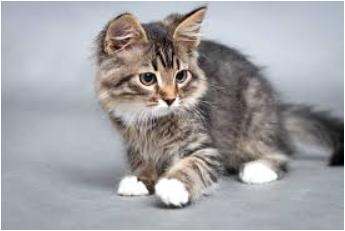
\includegraphics[scale=0.7]{images/telechargement.PNG}
        \caption{Chat de Google Images}
        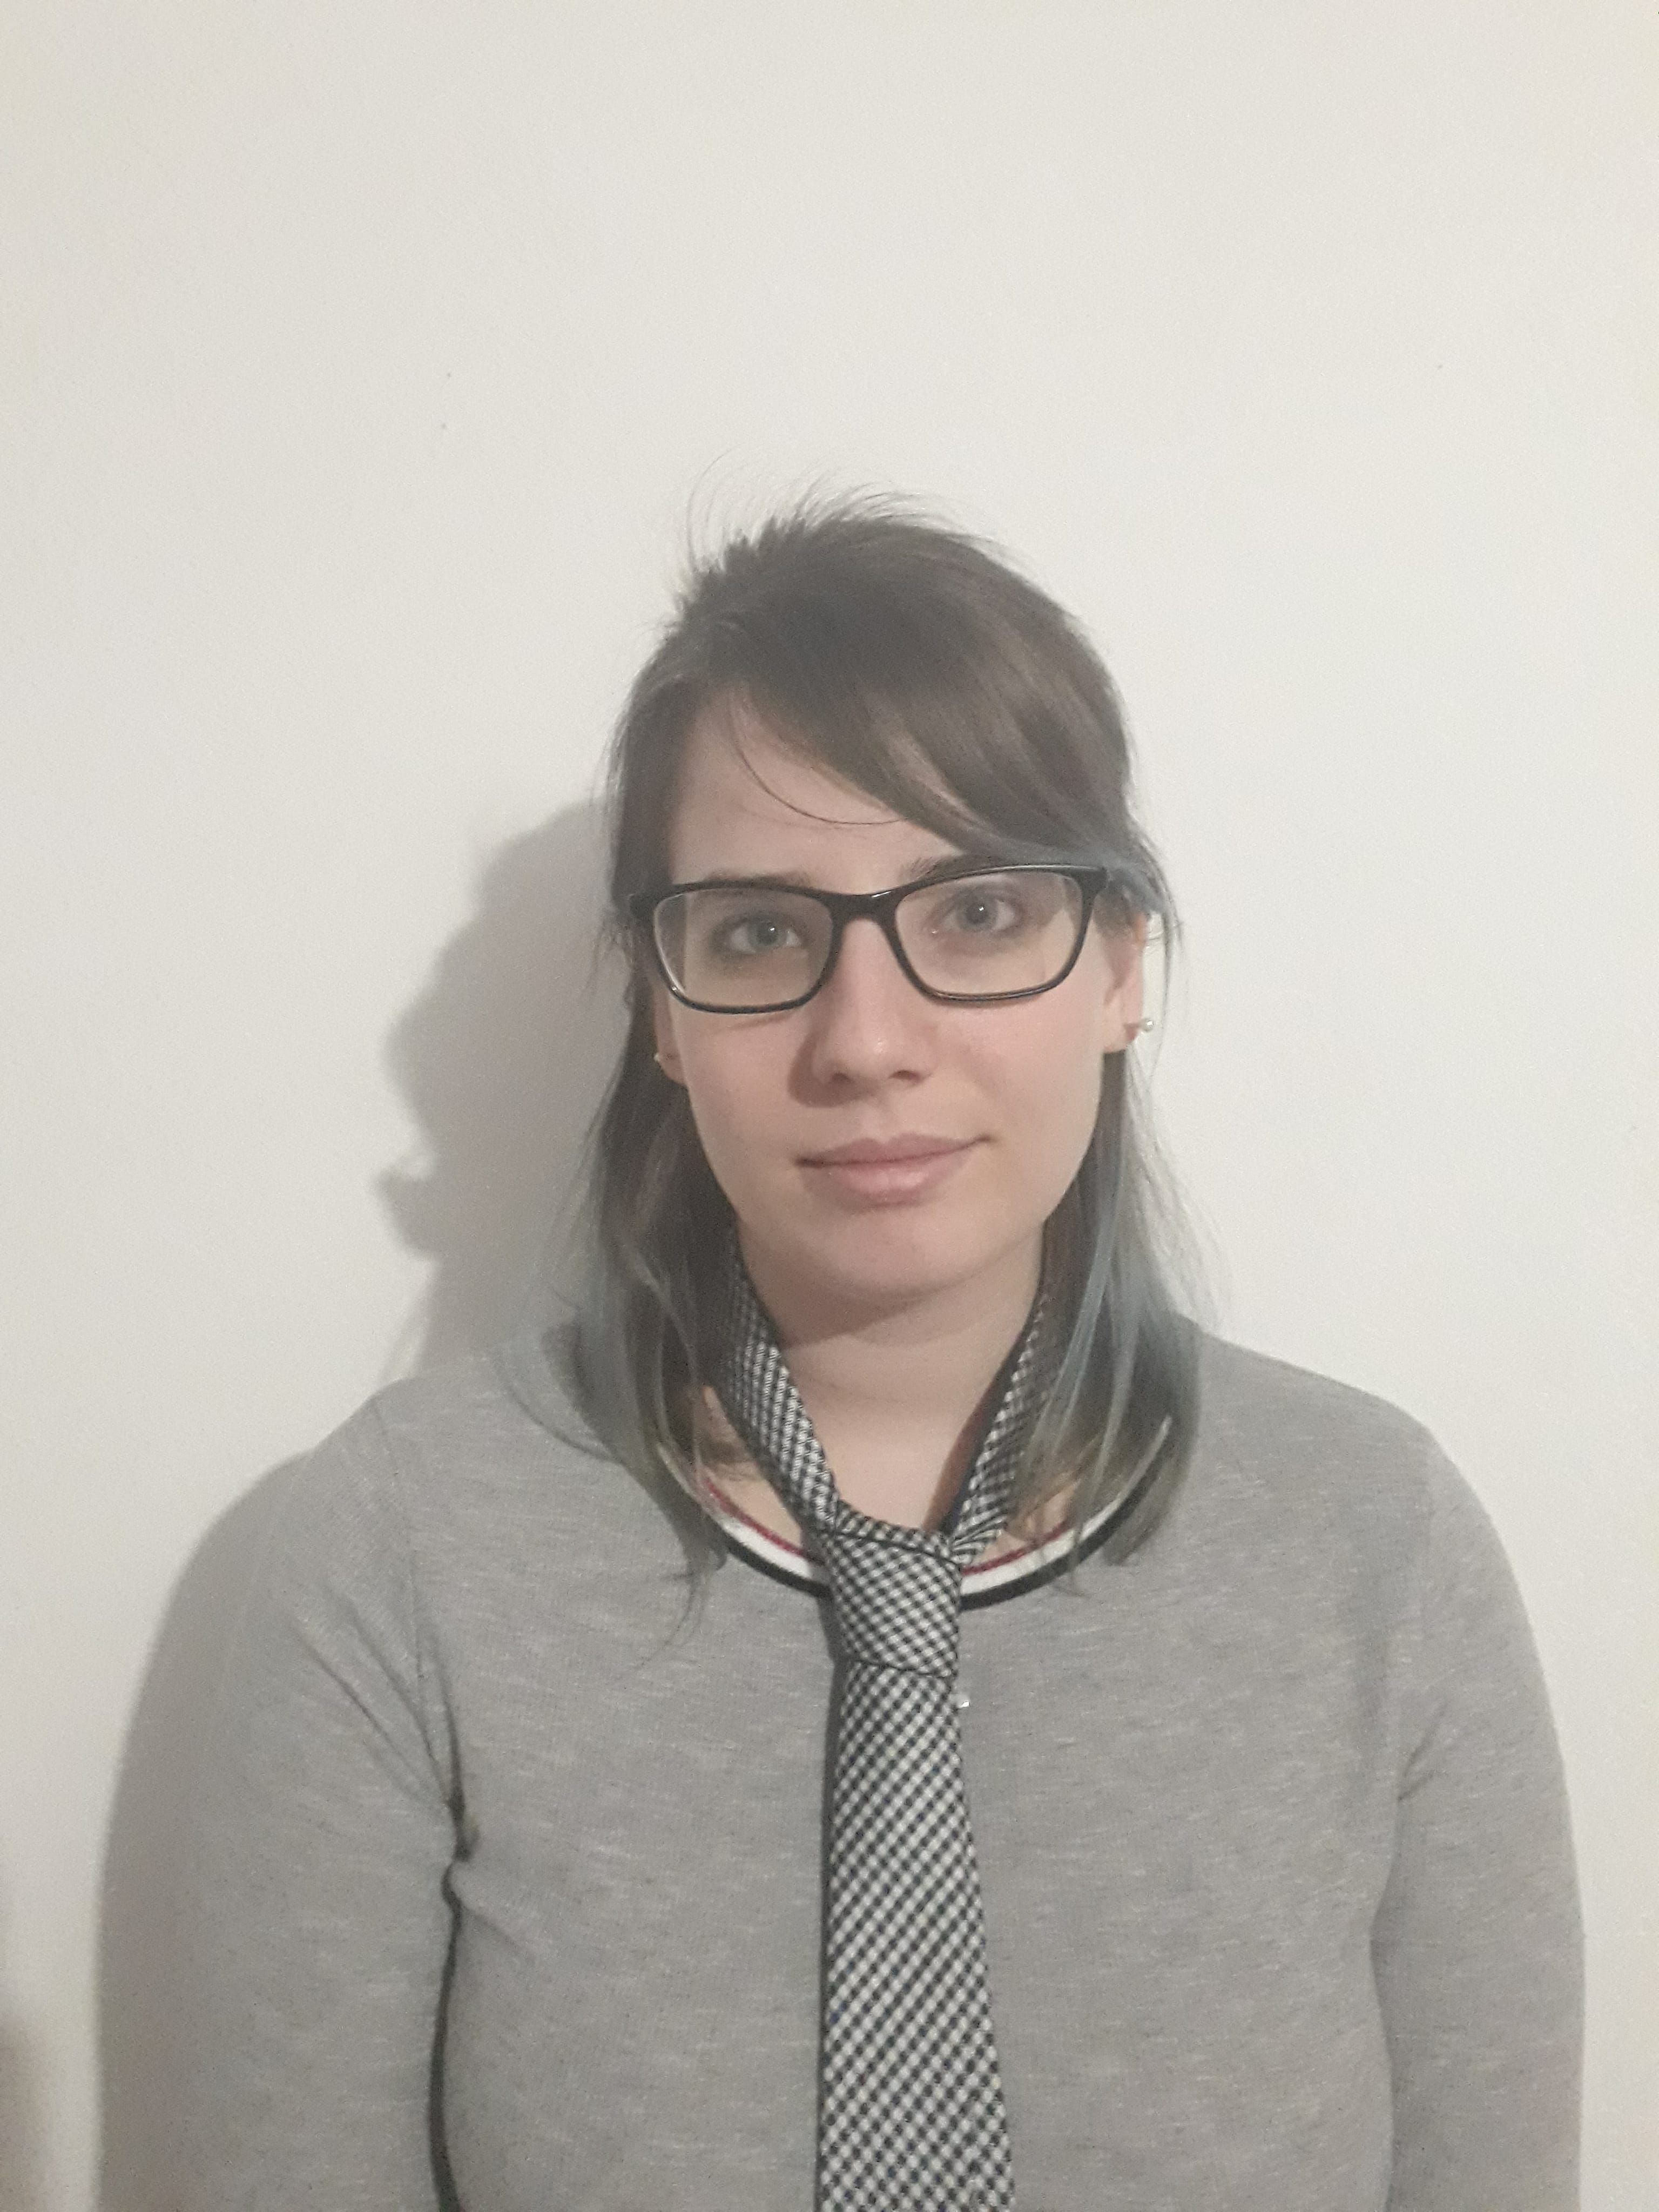
\includegraphics[scale=0.04]{images/27785203_330504664108478_1945544054_o.jpg}
        \caption{Photographie de Nathanaëlle VILLER}
    \end{figure}
En utilisant l'image de chat dans la recherche de Google Image on obtient le résultat ci-dessous. (Figure 3) Nous pouvons constater qu'il retourne les sites utilisant l'image fournis et qu'il propose de chercher les images similaires.  Malheureusement, cette recherche va "traduire" en mots clefs notre image initiale pour fournir des images peu similaires. Voir Annexe 1.

    \begin{figure}[!ht]
    \centering
        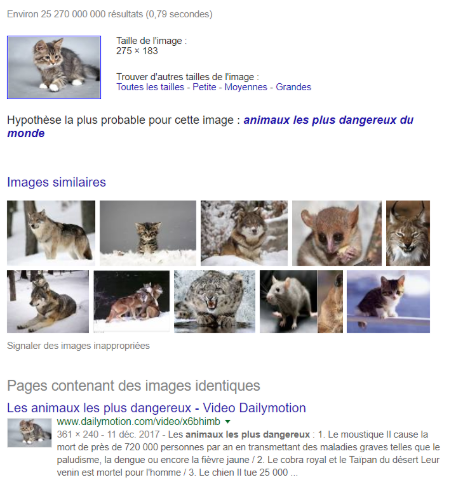
\includegraphics[scale=1]{images/ResGI.PNG}
        \caption{Résultat de la recherche via une image sur Google}
    \end{figure}

Le résultat des images similaires fourni par Google avec la photographie en Figure 2 n'est pas plus concluant non plus. (Figure 4) En effet, Google va aussi "traduire" la photographie en un mot clef : girl, et ressort des images de femmes et d'hommes. Les photographies sont similaires dans leur style. On peut voir qu'il y a une personne sur un fond en général unique mais en rien ces personnes ne ressemblent à Nathanaëlle VILLER.
    \begin{figure}[!ht]
    \centering
        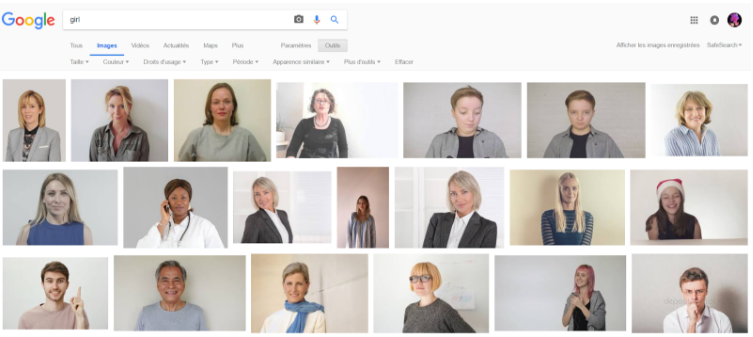
\includegraphics[scale=0.7]{images/Res3GI.PNG}
        \caption{Résultat de la recherche des images similaires par Google pour la Figure 2}
    \end{figure}
    
\subsubsection{Site de recherche de sosie}
Il existe quelques sites permettant de chercher son sosie. L'un des plus connus est twinstrangers.com. Ce site demande une photo, ainsi que quelques informations comme la date de naissance et le genre. Le site retourne ensuite la personne avec le plus de similitudes. Pour accéder au suivant, il faut payer. 
Voir Annexe 2 pour les 3 premiers résultats obtenus à partir de la photographie en Figure 2. 
    
Il s'agit de jeunes filles d'un âge plus ou moins proche de Nathanaëlle, leurs yeux sont également clairs et elles portent des lunettes. Mais on ne peut pas parler de sosie. 
D'après les termes d'utilisations du site, nous pouvons apprendre que seul le visage (à partir de la photo) sert à faire la recherche. Cette dernière sera faite parmi la base de données du site. Rien n'est dit par rapport au genre, mais puisqu'il faut le renseigner nous pouvons nous questionner si ce dernier ne permettait pas de faire un premier filtre. Ce site a pour but de permettre à des sosies de se trouver puis de se rencontrer. Cette plate-forme se limite à une base de données interne et à des personnes physiques, ce qui est différent de notre objectif.
Mais il semble intéressant d'étudier comment fonctionne l'algorithme de ce site. 
\\\\
Il existe d'autres sites tels que pictriev.com qui déduit si nous sommes un homme ou une femme ainsi que notre âge et nous fournis les célébrités auxquelles nous ressemblons le plus. Nous pouvons constater en annexe 3 que ce dernier n'est pas au point. Il en va de même pour celebslike.me (annexe 4). Tous les 2 sont des sites permettant de chercher son sosie parmi les personnalités connues. Encore une fois cela ne va pas avec nos objectifs. Au vu des résultats, les algorithmes d'être performant.

\subsubsection{Google Arts \& Culture}
Google Arts \& Culture est une application américaine qui permet de trouver son sosie en oeuvre d’art. Google Arts \& Culture a collaboré avec plus de 1 200 musées, galeries et institutions de 70 pays pour rendre leurs expositions accessibles à tous en ligne, sûrement aussi pour avoir une base de données interne à interroger. Malheureusement cette fonctionnalité "trouver son double dans une oeuvre d'art" de l'application n'est disponible qu'aux États unis et un test n'a donc pas pu être possible. Mais nous pouvons trouver des articles qui en parlent. Le fonctionnement est simple, il suffit de charger une photographie ou un autoportrait et l'algorithme va analyser les traits du visage à plus de 70 000 portraits provenant de collection du monde entier. Twitter a été rempli de test des internautes américains dont voici un exemple bluffant (Figure 5).
\begin{figure}[!ht]
    \centering
        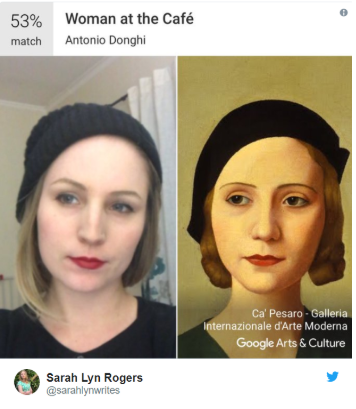
\includegraphics[scale=1]{images/GAC.PNG}
        \caption{Exemple trouvé sur Twitter}
    \end{figure}

La technologie de reconnaissance faciale FaceNet développée par Google, utilisée dans cette application est désormais disponible dans une version open source officieuse, OpenFace. Cette dernière est très intéressante pour notre sujet de recherche. Les résultats obtenus par l'application sont concluants et l'on observe des similitudes entre les deux photographies. Il s'agit de la première application connue permettant de trouver son sosie avec une oeuvre d'art. Ce qui rejoint fortement notre objectif bien que se limitant à des oeuvres d'art.  

\subsubsection{Les sites de rencontre}
Les sites de rencontrent se mettent de plus en plus dans la recherche de sosie. L'objectif est de permettre aux internautes de chercher un sosie de leur célébrité préférée ou de leur ex-partenaire ou de la personne leur plaisant mais étant déjà prises. Dans les sites de rencontre permettant ce genre de recherche nous pouvons citer Badoo et Match (Meetic). 
Badoo est assez frappant car les similitudes trouvées sont fortes (même si certains correspondent à de faux comptes usurpant la photo d'une autre personne). (Figure 6)
\begin{figure}[!ht]
    \centering
        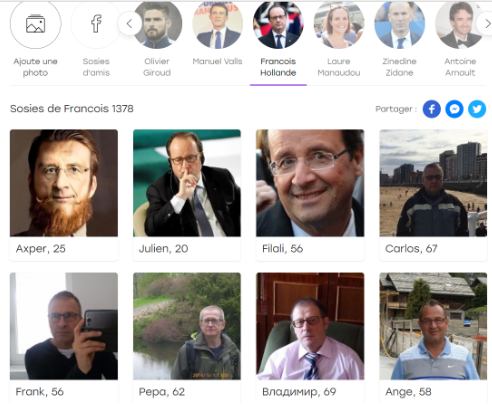
\includegraphics[scale=1]{images/badoo.PNG}
        \caption{Exemple avec Badoo}
    \end{figure}
    
\subsubsection{Conclusions sur ces solutions}

Actuellement, les solutions permettent surtout de trouver un sosie de nous-mêmes avec une personne physique. Mais aucune d'entre elles n'est une solution probante. Il existe des solutions (application ou site web) mais en général elles se servent dans leur base de données locale et pas "sur internet" en règle générale. 

Ce qui manque à ces applications : 
\begin{itemize}
    \item Une recherche à travers internet 
    \item Une sortie de sosie qui ne soit pas uniquement une personne physique réelle 
    \item Une reconnaissance morphologique en plus de celle faciale
\end{itemize}

Pour ce qui est du second point, Google a développé un algorithme permettant de chercher un sosie avec une oeuvre d’art de type peinture ou dessin exposé dans un musée. Il faudrait donc trouver une solution pour proposer un outil à plus large spectre, qui reprendrait l’existant mais pour le mener plus loin. 
Ouvrir le retour de sosie à toute oeuvre : peinture, dessins, coloriage, photographie … Pour trouver une personne physique ou un personnage fictif en termes de sosie. Et, effectuer la recherche en dehors d'une base de données locale mais s'appuyer sur toutes les ressources dont dispose internet. 

\subsection{Besoins utilisateurs}
Suite à notre étude il est ressorti deux grands besoins utilisateurs. Le premier étant de pouvoir trouver son sosie et l'autre de pouvoir aider à compléter la base de données. Et cela rentre bien avec l'objectif d'avoir une solution simple. La solution pourrait être proposée sur différente plate forme : un site web et une application sur les différents supports mobiles. Pour permettre aux gens d'avoir un avant-goût de l'application et leur donner envie de l'utiliser, cette dernière pourrait être utilisée de façon réduite sans avoir besoin de s'enregistrer. 
\\ Partir sur une base de données collaborative est envisageable car, 84\% sont d'accord de partager leurs oeuvres à l'application si ces dernières servent uniquement à la recherche de sosies et qu'elles ne sont pas détournées de l'application. On peut voir cela comme une forme de partenariat: les artistes remplissent notre base de données et en échange nous leur permettons de se faire connaître. Cela permet d'avoir une seconde source de provenance pour remplir la base en plus de la fouille de données. 
\\De plus, notre proposition de pouvoir trier sa recherche de sosie (par genre : bande dessinée, comic, manga, ...) a fort plu au vu du résultat de notre étude : 90,6\% répondent "Oui" à la question : "Aimeriez vous avoir la possibilité de choisir la catégorie de recherche ?"  

\subsection{Fouilles de données}
Pour la partie fouilles de données, nous utiliserons un algorithme de crawling web, ou en français, robot d'indexation.
Il s’agit de bots logiciels qui vont parcourir les sites internet avec
pour objectif principal de les indexer. Le parcours se fait en profondeur, le
logiciel accédant tour à tour à chaque pages ou sites externe grâce aux liens
hypertextes présents dans la page en cours d’analyse (exemple : lien URL) puis
réitère l’opération. On peut ajouter des paramètres au bot afin qu’il recherche
en même temps que sa "lecture". Dans notre cas, l'objectif sera de récupérer les images de certains sites ainsi que quelques informations liées à l'image (auteur, univers, etc.).

On trouve facilement plusieurs crawler tel que :
\begin{itemize}
    \item \textbf{GoogleBot} est le crawler le plus connu. Il permet d’indexer les sites
internet. Il fait principalement de la "lecture" de site. Dans notre cas c'est insuffisant puisque l'on veut faire une recherche dans les sites parcourus. 
Dans le même ordre d’idée, nous pouvons retrouver les bots des moteurs
de recherche tels que BingBot, Slurp Bot (Yahoo), DuckDuckBot,
BaiduSpider (Baidu est un moteur de recherche en chinois) ou encore
YandexBot (utilisé pour les moteurs de recherches russes).
\item \textbf{Facebook External Hit}, Facebook utilise ce crawler afin de permettre
à ces utilisateurs, lorsqu’ils envoient (publient) un lien internet
à un autre utilisateur du site, de récupérer et afficher certaines
informations importantes par exemple : des extraits vidéos,
des images ou des titres.
Ce bot ne correspond pas à ce que nous souhaitons mettre en place.
Par contre il pourrait être un élément de réponse à la question des
droits d’auteurs. En effet, si l’outil était développé concrètement comment
renvoyer l’image trouvée ainsi que toutes ses informations sans
enfreindre les lois sur le droit à l’image ? Avec ce type de bot, cela est
possible car il permet de récupérer et afficher l’information choisie et
de renvoyer vers sa localisation dans la toile.
\item \textbf{HTTrack} est un logiciel aspirateur de site internet qui crée des miroirsdes sites Web pour une utilisation hors ligne.
\item \textbf{Alexa Crawler} (développé par Amazon) va indexer les sites après
les avoirs triés en fonctions de certains critères. Cela se rapproche de ce que nous souhaitons en apportant une dimension de classement selon des critères multiples qu’il est possible de sélectionner et filtrer.
\item \textbf{Nutch} est un crawler destiné à un moteur de recherche open source.
Son architecture est modulaire et permet de créer des plugins pour différentes phases du processus : récupération des données, analyse des documents, recherche, etc. Nutch est le crawler qui se rapproche le plus de la solution que nous
cherchons.
\end{itemize} 
\subsection{Traitement et comparaison d'images}
Ce qui est actuellement le plus courant est la comparaison faciale. La dernière technologie permettant de comparer des photographies avec des images est FaceNet. Ce dernier correspond exactement a ce que nous cherchons. 
Pour ce qui est de la morphologie, il n'existe pas encore d'algorithme efficace. Le plus simple restant la comparaison par pixel. 

En mai 2015, Benjamin Billet a justement publié un article sur les différentes méthodes les plus connues et pratiquées pour la recherche d'image similaire. La comparaison d'image par empreinte ne permet pas d'obtenir de résultats concluants, car, elles cherchent à obtenir un identifiant par rapport aux couleurs et à leur disposition sur l'image et nullement sur des caractéristiques morphologiques. Le but étant de trouver des copies conforme entre images. 

Par contre un histogramme de couleurs en moyenne pas bloc nous permettrait de comparer nos images pour trouver les plus proches. 

\textbf{Histogramme des couleurs}
Un histogramme des couleurs représente la distribution des couleurs dans l'image, c'est-à-dire le nombre de pixels dont la couleur appartient à une plage donnée, les différentes plages couvrant la totalité de l'espace colorimétrique (voir cet exemple très parlant). L'histogramme nous donne donc une représentation statistique de l'image, deux images étant analysées en comparant leurs histogrammes. Cette méthode, bien que très simple à implémenter, présente toutefois le désavantage d'être purement colorimétrique : en pratique, deux images aux sujets très différents peuvent avoir des histogrammes très proches.

\textbf{Moyenne par bloc}
Cette méthode est elle aussi assez simple et consiste à diviser l'image en blocs et à calculer la moyenne colorimétrique de chaque bloc. La comparaison se fait en calculant la moyenne des différences de couleur entre les blocs de chaque image, sous réserve que les deux images aient été hashées avec le même nombre de blocs. 
\\\\
Actuellement, les technologies développées permettent de comparer des images dans leur ensemble, de trouver celles identiques (grâce à une empreinte), ou de trouver un visage et de le comparer. La partie sur la morphologie est encore en recherche. On peut trouver des thèses traitant le sujet, mais pas de solution concluante développée. Ainsi pour notre problématique, si nous voulons comparer la morphologie de 2 personnes/personnages il nous faudra attendre une avancée technologique. 
\\\\
Alors, comment, à partir de la reconnaissance faciale et de la fouille de données, peut-on identifier l’ensemble des sosies potentiels d’une personne ?

\section{Solution Architecturale}
Aujourd'hui il n'existe pas de solution à notre problématique. Voici donc une proposition d'architecture qui y répond. 

\begin{figure}[!ht]
    \centering
        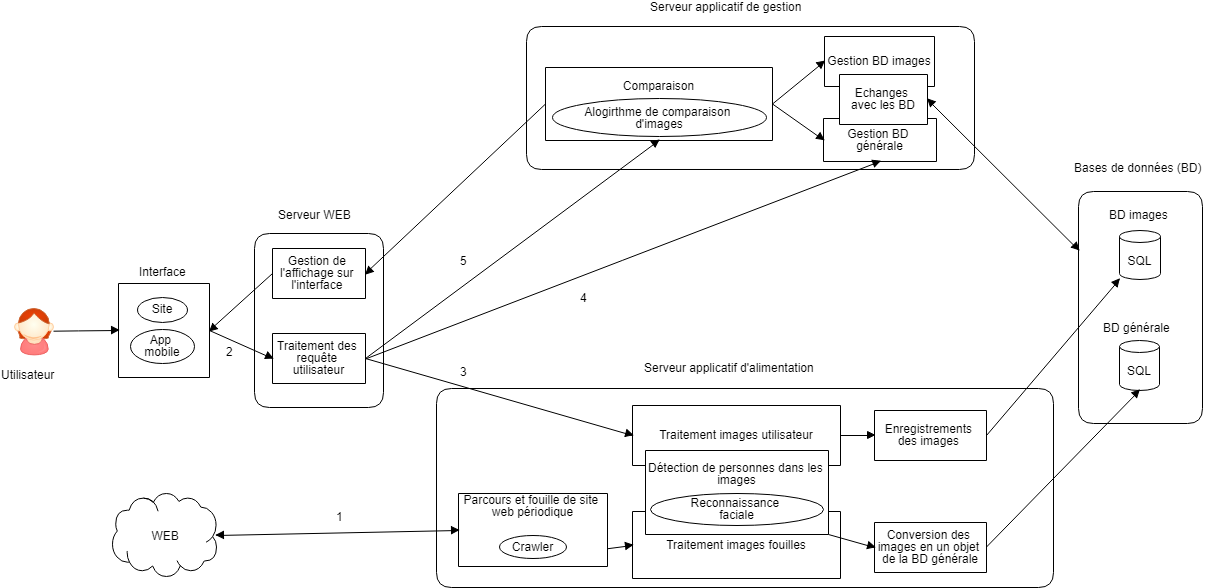
\includegraphics[scale=0.4, angle=-90]{images/SchemaArchitecture.png}
        \caption{Architecture de notre solution}
    \end{figure}

    
 \subsection{Fouilles périodique} 
 En utilisant un crawler, l'algorithme va parcourir différents sites web et récupérer les différentes images trouvées. Il faudra ensuite trier les images pour ne garder que celles nous intéressant : celles contenant une personne/ un personnage. Pour cela on utilisera la reconnaissance faciale, ainsi l'on pourra écarter les images ne contenant aucun portrait et celles contenant plusieurs portraits. Les images conservées seront converties en un "code" permettant ensuite leurs comparaisons et seront enregistrées avec toutes sortes d'informations récupérées sur le site, comme son URL. Attention on n'enregistre pas l'image par contre, uniquement ses informations et le "code" produit par notre algorithme. Tout ceci sera enregistré dans la base de données générale de l'application. 
 \subsection{Actions utilisateur}
 L'utilisateur aura 3 types d'action possible via l'interface. 
 \begin{itemize}
     \item \textbf{Gestion utilisateur} : Il y aura toutes les actions liées à la gestion du compte utilisateurs tel que la création de comptes et la modification de se dernier. 
     \item \textbf{Ajout d'images} : Un utilisateur pourra ajouter une image à son compte, sans cela il ne pourra pas faire de recherche de sosies. Mais il pourra aussi ajouter des images pour remplir de façon collaborative la base de données de l'application. 
     \item \textbf{Recherche de sosie} : L'utilisateur pourra faire une recherche de sosies de façon générale ou spécifique grâce à la fonctionnalité de tri permettant de chercher un sosie de en fonction d'univers précis. 
 \end{itemize}
 \subsection{Enregistrements d'images utilisateur}
 En plus de récupérer des images via un crawler sur le web, la base de données pourra être remplie de façon collaborative par les utilisateurs. Toutes les images uploader par les utilisateurs sur l'application seront testés pour vérifier qu'il s'agit bien d'une personne grâce à la reconnaissance faciale et ensuite elles seront aussi converties un "code" pour être enregistré dans la base de données. Par contre, à l'inverse des images récupérées sur les sites web parcourus, ces images seront enregistrées en local dans une base de données image. Ainsi chaque "code" sauvegardé dans la base de données générale référencera une image enregistrée dans la base de données image. 
 \subsection{Gestions utilisateur}
 Les modifications que l'utilisateur souhaitera apporter en dehors du changement de sa photo seront transcrites en requête envoyée à la base de données.  Cela permettant la création, récupération, modification et suppression d'un compte. 
 \subsection{Comparaison}
 La comparaison se fait sur la photographie liée au compte de l'utilisateur. Grâce à un algorithme de comparaison d'image, les différents "codes" de chaque image seront comparés. On en gardera les meilleurs résultats pour ensuite les afficher. Les différents types d'algorithmes de comparaison d'images transcrivent la plupart du temps les images en un "code", c'est ce dernier qui permet la comparaison et de savoir si les images sont complémentaires et à combien de pourcentage. Pour plus d'exactitude dans la comparaison, on peut aussi comparer les visages entre eux. Grâce à la reconnaissance faciale, il faudrait récupérer la zone du visage, voir la tête tout entière et comparer ces deux zones entre elles pour voir le complémentarité. Au même titre il faudrait pouvoir comparer la morphologie de chacun. Mais pour l'heure il n'existe pas de "reconnaissance morphologique" aboutie en termes d'algorithme. 

\subsection{Affichage}
L'affichage des images enregistrées dans la base de données image pourront simplement être affichées. Pour ce qu'y est des images récupérées sur la toile on pourrait utiliser le système de Facebook, permettant d'afficher une miniature de l'image et un lien cliquable vers le site et l'image. Ou alors nous pourrions afficher dans notre page la page internet du site hébergeant l'image. 
\subsection{Contraintes légales}
Pour éviter les problèmes de droits d'auteurs, nous ne pouvons pas enregistrer en local les images trouvées sur les sites web. Comme notre objectif est de comparer les images, il suffit de "convertir" l'image en un code. Ce code que nous obtenons peut, lui, être enregistré en local. Pour retrouver et afficher l'image nous ne garderons d'elle que le lien URL pour la retrouver. \\ \\
Dans la législation française, le droit d'auteur permet à un auteur de choisir de quelle manière si son oeuvre peut être partagée, reproduite, réutiliser ... D'un auteur à l'autre, ses autorisations changent. Enregistrer une image pour la partager à un public dans le cadre de notre application peut être illégal en fonction des droits décider par les auteurs. Par contre référencer les sites où ont été partagées ces images n'est pas une infraction. \\ 
De plus, les articles 226-1 à 226-8 du Code civil précisent que « tout individu jouit d’un droit au respect de sa vie privée ainsi que d’un droit à l’image. En vertu de ces dispositions, il va de soi que la publication ou la reproduction d’une image (photographie ou vidéo) sur laquelle une personne est facilement reconnaissable n’est autorisée qu’avec son consentement préalable, et ce, que l’image soit préjudiciable ou non. Nous ne pouvons donc pas nous permettre de réutiliser des photographies librement dans notre application. \\ 
La solution qu'utilise Facebook est donc a exploité. Quant aux images uploadées par les utilisateurs, il suffira de leur faire accepter le droit de diffusion dans l'application de leurs images et photographies. 

\newpage
\addcontentsline{toc}{section}{Conclusion}
\section*{Conclusion}
Il n'existe à ce jour, aucune solution permettant de trouver de chercher son sosie parmi des personnes imaginaires. Il existe des solutions plus ou moins réussis qui permettent de trouver son sosie parmi des être humains réelles ou parmi des stars. Mais dans le domaine du fictif le marché est encore jeune et la concurrence est faible. Pour l'instant une seule application réussi a été recensé et ne fonctionne que pour les oeuvres d'art. 
\\ \\ 
Du côté du public les retours sont positifs. Les gens sont de nature curieuse et pense que que notre solution serait un bon amusement. Quant à la communauté cosplay, une telle solution apporterait une aide précieuse et permettrait de développer la communauté. 
\\ \\
La grande majorité des solutions existantes sont privés, nous ne pouvons donc pas récupérer leur méthodologie. Suite à notre réflexion, grâce à notre solution architecturale il devrait être possible de créer une application répondant à notre besoin. 
\\ \\ 
Pour ce qui est de la comparaison morphologique il faudra par contre attendre un développement plus poussé des technologies et algorithme actuel ou bien tester des solutions proposées dans certaines thèses. 
\newpage



\section{Annexes}
Annexe 1 : 
\begin{figure}[!ht]
    \centering
    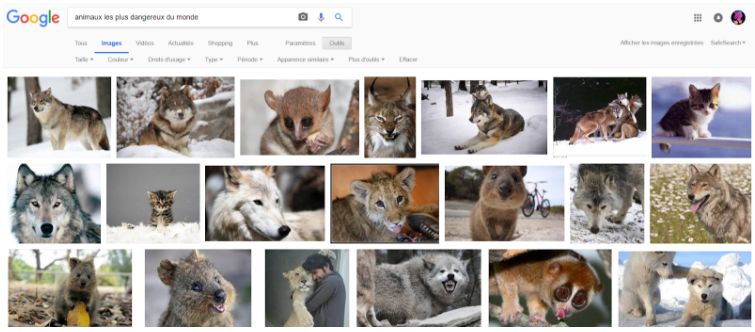
\includegraphics[scale=0.8]{images/Res2GI.PNG}
    \caption{Résultat de la recherche des images similaires par Google pour la Figure 1}
\end{figure}

Annexe 2 : 
\begin{figure}[!ht]
    \centering
        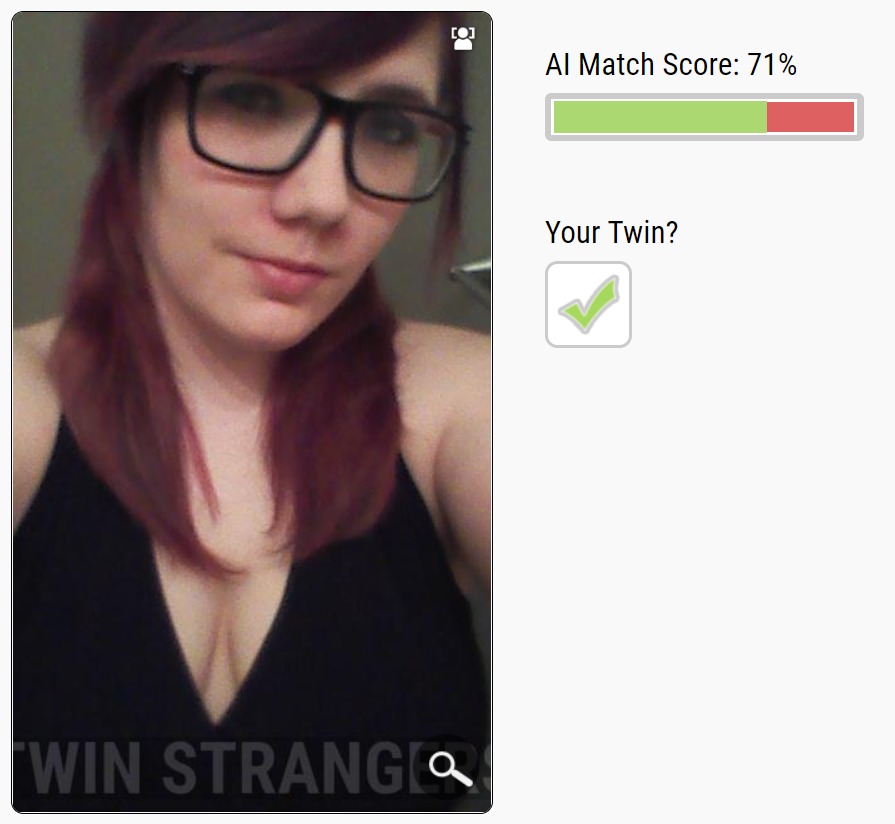
\includegraphics[scale=0.45]{images/ResS1.PNG}
        \caption{Premier sosie}
    \end{figure}
    \begin{figure}[!ht]
    \centering
        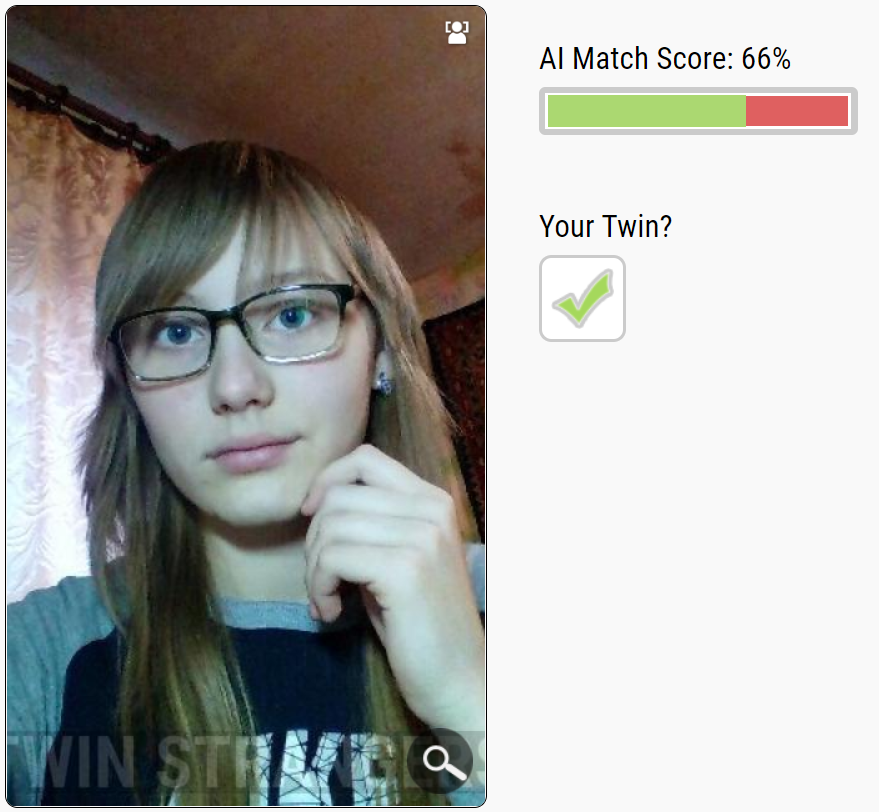
\includegraphics[scale=0.3]{images/ResS12.PNG}
        \caption{Deuxième sosie}
    \end{figure}
\begin{figure}[!ht]
    \centering
        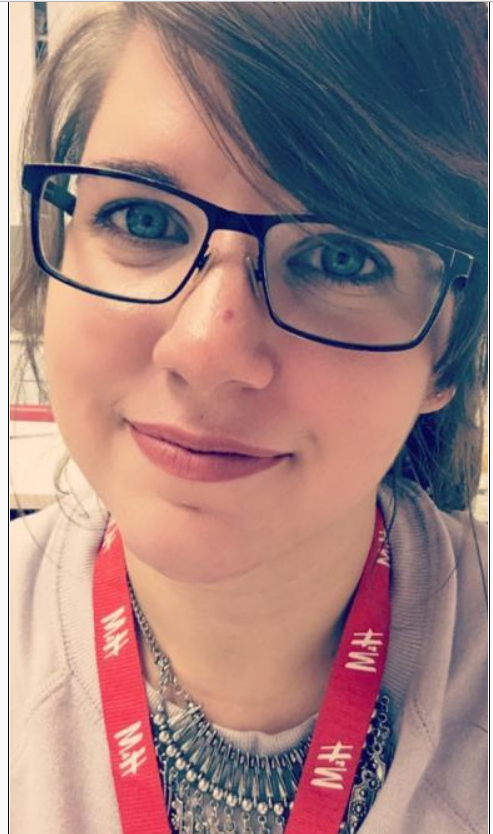
\includegraphics[scale=0.3]{images/ResS13.PNG}
        \caption{Troisième sosie}
    \end{figure}
    
  \newpage
Annexe 3 : 
\begin{figure}[!ht]
    \centering
        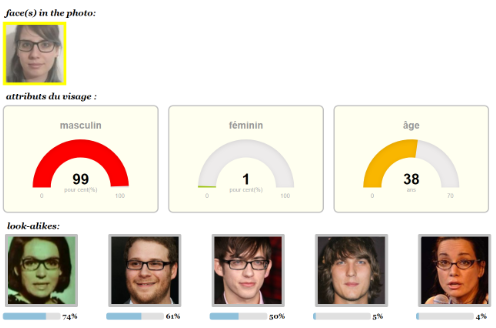
\includegraphics[scale=1]{images/ResS2.PNG}
        \caption{Résultat du second site}
    \end{figure} 
\newpage
Annexe 4 :
\begin{figure}[!ht]
    \centering
        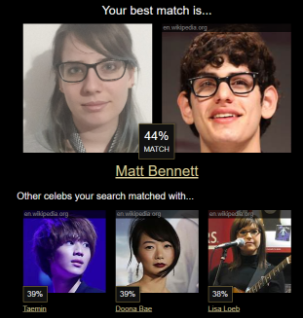
\includegraphics[scale=1]{images/ResS3.PNG}
        \caption{Résultat du troisième site}
    \end{figure}
\newpage
Sources : 
\begin{itemize}
    \item \textbf{TinEye} - \textit{Moteur de recherche d'image} -         \url{http://labs.tineye.com/multicolr/}
    \item \textbf{Google} - \textit{Moteur de recherche d'image} - \url{https://www.google.fr/}
    \item \textbf{TWIN STRANGERS} - \textit{Site de recherche de sosie} - \url{http://www.twinstrangers.com/}
    \item \textbf{PicTriev} - \textit{Site de recherche de sosie} - \url{http://www.pictriev.com}
    \item \textbf{CelebsLike.Me} - \textit{Site de recherche de sosie} - \url{http://www.celebslike.me/}
    \item \textbf{Badoo} - \textit{Site de rencontre} - \url{https://badoo.com/}
    \item \textbf{Match / Meetic} - \textit{Site de rencontre} - \url{https://www.meetic.fr/}
    \item \textbf{Numerama} - \textit{Article sur la reconnaissance faciale} - \url{https://www.numerama.com/tech/126861-openface-un-script-de-reconnaissance-faciale-open-source.html}
    \item \textbf{Medium} - \textit{Article sur la reconnaissance faciale} - \url{https://medium.com/@vinayakvarrier/building-a-real-time-face-recognition-system-using-pre-trained-facenet-model-f1a277a06947 }
    \item \textbf{IDEMIA } - \textit{Article sur la reconnaissance faciale } - \url{https://www.morpho.com/fr/reconnaissance-faciale }
    \item \textbf{OpenFace API Docs} - \textit{Documentation de OpenFace} - \url{http://openface-api.readthedocs.io/en/latest/}
    \item \textbf{u Ottawa } - \textit{Article sur le crawling} - \url{http://ssrg.site.uottawa.ca/docs/CASCON2013.pdf }
    \item \textbf{Oncrawl } - \textit{Article sur le crawling } - \url{http://fr.oncrawl.com/2016/introduction-crawler-web/}
    \item \textbf{Business to web } - \textit{Article sur le crawling } - \url{https://www.b2w.fr/1489-quest-ce-crawl.html}
    \item \textbf{Définitions marketing } - \textit{Article sur le crawling } - \url{https://www.definitions-marketing.com/definition/robot-d-indexation/ }
    \item \textbf{Keycdn } - \textit{Article sur le crawling} - \url{https://www.keycdn.com/blog/web-crawlers/}
    \item \textbf{Benjamin Billet} - \textit{Comparaison d'images} - \url{http://benjaminbillet.fr/blog/index.php?article1/detection-images-similaires }
    \item \textbf{CFC Centre Français d'exploitation du droit de Copie} - \textit{Droit d'auteur} - \url{http://www.cfcopies.com/juridique/droit-auteur }
    \item \textbf{economie.gouv.fr} - \textit{Droit d'auteur} - \url{https://www.economie.gouv.fr/files/files/directions_services/apie/propriete_intellectuelle/publications/utiliser_contenu_etapes_essentielles.pdf }
    \item \textbf{Service Public} - \textit{Droit d'auteu}r - \url{https://www.service-public.fr/professionnels-entreprises/vosdroits/F23431 }
    
    
    
    \item \textbf{ } - \textit{ } - \url{ }
    
    
\end{itemize}



%\subsection{}
%\subsubsection{}

%\begin{itemize}
%\item	
%\item	
%\item
%\item	
%\item	
%\end{itemize}


%\begin{center}
%		    \includegraphics[scale=0.6]{images/cas_utilisation}	
%		\end{center}
	


%\begin{verbatim}

\end{document}
